% =================================================================================
% Hier ausw�hlen, ob TUD-Design oder nicht
% =================================================================================
\newif\ifTUDdesign
\TUDdesigntrue					% TUD-Design
%\TUDdesignfalse				% F�r Rechner ohne installierte TUDdesign-Pakete
% =================================================================================


% =================================================================================
% Hier Daten f�r studentische Arbeit eingeben
% =================================================================================
\newcommand{\SADATyp}{Praktikumsbericht}
\newcommand{\SADATitel}{Versuch I, Modellbildung und Simulation eines Doppelpendel-Systems}
\newcommand{\SADAStadt}{Darmstadt}
\newcommand{\SADAAutor}{Andreas Jentsch, Ali Kerem Sacakli}
\newcommand{\SADABetreuer}{}
\newcommand{\SADABetreuerII}{}
\newcommand{\SADABetreuerIII}{}
\newcommand{\SADABegin}{}
\newcommand{\SADAAbgabe}{Praktikum Matlab/Simulink II}
\newcommand{\SADASeminar}{}
% =================================================================================


% =================================================================================
% Auswahl des IAT-Fachgebiets (rtm / rtp)
% =================================================================================
\newif\ifrtm
\rtmtrue	% rtm
%\rtmfalse	% rtp
% =================================================================================


% =================================================================================
% Erkl�rung, dass die Arbeit ohne Hilfe Dritter etc. erstellt wurde
% =================================================================================
\def\SADAVarianteErklaerung{ETIT}		% FB 18, Elektrotechnik
%\def\SADAVarianteErklaerung{MBDA}		% FB 16, Maschinenbau, Diplomarbeit
%\def\SADAVarianteErklaerung{MBSA}		% FB 16, Maschinenbau, Studienarbeit
% =================================================================================


% =================================================================================
% Ausnahmen von der automatischen Silbentrennung
% =================================================================================
\hyphenation{Aktu-ali-sie-rung Screen-shots Pa-rallel-ro-bo-ter Zu-stands-raum-mo-del-le nach-voll-zieh-bar Pro-jekt-se-mi-nar}
% =================================================================================


% =================================================================================
% Hier NIICHTS �ndern!
% =================================================================================
\ifTUDdesign
	\documentclass[11pt, twoside, colorback, accentcolor=tud2c, nopartpage, bigchapter, fleqn, ngerman, longdoc]{tudreport}
\else
	\documentclass[11pt, a4paper, twoside, fleqn, ngerman]{scrreprt}
  % F�r Entwurf auf Rechnern ohne installierte TUDdesign-Pakete	
	\usepackage{exscale}	% Korrektur math-Zeichen
	\usepackage{eurosym}
\fi
%eps-plot von Matlab in pdf umwandeln, um diese einbinden zu k�nnen
\usepackage{epstopdf}
%Paket listings f�r das Einbinden von Quelltext
\usepackage{listings}
%Stil Matlab_colored definieren
\lstdefinestyle{Matlab_colored}
{
	language = Matlab,
	tabsize = 4,
	framesep = 3mm,
	frame = tb,
	classoffset = 0,
	basicstyle = \ttfamily,
	keywordstyle = \bfseries\color[rgb]{0,0,1},
	commentstyle = \itshape\color[rgb]{0.133,0.545,0.133},
	stringstyle = \color[rgb]{0.672,0.126,0.941},
	extendedchars = true,
	breaklines = true,
	prebreak = \textrightarrow,
	postbreak = \textleftarrow,
	numbers = left,
	numberstyle = \tiny,
	stepnumber = 5	
}


\input{common/includes.tex}				% verwendete Pakete einbinden
\input{common/setup.tex}					% LaTeX-Einstellungen
\input{common/commonmacros.tex}		% oft verwendete Befehle
% =================================================================================


% =================================================================================
% Hier beginnt das eigentliche Dokument
% =================================================================================

\begin{document}
%\input{common/preface.tex} % Titelseite, Aufgabenstellung, Erkl�rung, Abstract, Inhaltsverzeichnis, etc.
\maketitle




% =================================================================================
% Anhang
% =================================================================================
%\appendix % Damit wird der Anhang begonnen. Die Kapitel werden ab jetzt mit Buchstaben nummeriert



% =================================================================================


%% =================================================================================
%% Abbildungsverzeichnis
%% =================================================================================
%\cleardoublepage
%\phantomsection					% F�r Aufnahme ins Inhaltsverzeichnis
%\addcontentsline{toc}{chapter}{\listfigurename}	% In Inhaltsverzeichnis von
%												% Dokument und pdf aufnehmen
%\listoffigures
%% =================================================================================
%
%% =================================================================================
%% Tabellenverzeichnis
%% =================================================================================
%\cleardoublepage
%\phantomsection					% F�r Aufnahme ins Inhaltsverzeichnis
%\addcontentsline{toc}{chapter}{\listtablename}	% In Inhaltsverzeichnis von
%												% Dokument und pdf aufnehmen
%\listoftables
%% =================================================================================

% =================================================================================
% Literaturverzeichnis
% =================================================================================
%\cleardoublepage
%\phantomsection					% F�r Aufnahme ins Inhaltsverzeichnis
%\addcontentsline{toc}{chapter}{\bibname}	% In Inhaltsverzeichnis von
%											% Dokument und pdf aufnehmen
%\bibliographystyle{gerabbrv}	% Verweise nummeriert in eckigen Klammern, alphabetisch sortiert
\bibliographystyle{gerunsrt}	% Verweise nummeriert in eckigen Klammern, nach Erscheinung sortiert

% =================================================================================

\setcounter{chapter}{1}

%Warum geht title/section nicht?
\section{Doppelpendel-System}
Im Praktikum Matlab/Simulink II werden weiterf�hrende Konzepte der Regelungstechnik basierend auf einem Doppelpendel-System erarbeitet. In diesem Versuch geht es um die Modellierung des Doppelpendelsystems durch verschiedene Modellierungsm�glichkeiten.

Der erarbeite Code f�r die symbolische L�sung der Bewegungsgleichungen f�r das Doppelpendel-System sieht wie folgt aus:

\lstinputlisting[style=Matlab_colored,caption={Code des Doppelpendel-Modells}, label={Code_Modell}]{Codes/V1_Modell.m}


\newpage

\section{Implementierung des Modells durch verschiedene Modellierungsm�glichkeiten}

Das im vorherigen Kapitel dargestellte Modell wird mit folgenden drei Modellierungsm�glichkeiten implementiert:
\begin{itemize}
	\item Fcn-Blocks,
	\item MATLAB-Function-Blocks 
	\item einer M-File S-Function
\end{itemize}

Im folgenden Abschnitt wird f�r jede Implementierung das Simulink-Schaltbild mit dem zugeh�rigen Code zur Simulation vorgestellt.


\subsection{Fcn-Blocks}

\begin{figure}[htbp]
	\centering
	\includegraphics[scale=0.6]{Bilder/Fcn_Block_Simulink.JPG}
	\caption{Implementierung mit Fcn-Bl�cken}
	\label{fig:fcn}
\end{figure}

Dabei lautet die Funktion von \textbf{Fcn}: \newline
$-(6*(4*Rp1*u(2)*l2 - 4*u(1)*l2 + 6*Rp2*u(2)*l1*cos(u(3) - u(4)) - 6*Rp2*u(5)*l1*cos(u(3) - u(4)) + (3*g*l1*l2*m2*sin(u(3) - 2*u(4)))/2 + (3*u(2)^2*l1^2*l2*m2*sin(2*u(3) - 2*u(4)))/2 + 2*u(5)^2*l1*l2^2*m2*sin(u(3) - u(4)) + 2*g*l1*l2*m1*sin(u(3)) + (5*g*l1*l2*m2*sin(u(3)))/2))/(l1^2*l2*(8*m1 + 15*m2 - 9*m2*cos(2*u(3) - 2*u(4))))$ \newline \\
%Fcn2 Block
und f�r den \textbf{Fcn1} Block lautet die Funktion:\newline
$(6*(4*Rp2*u(2)*l1*m1 - 6*u(1)*l2*m2*cos(u(3) -u(4)) + 12*Rp2*u(2)*l1*m2 - 4*Rp2*u(5)*l1*m1 - 12*Rp2*u(5)*l1*m2 + 6*u(2)^2*l1^2*l2*m2^2*sin(u(3) - u(4)) - 3*g*l1*l2*m2^2*sin(u(4)) + (3*u(5)^2*l1*l2^2*m2^2*sin(2*u(3) - 2*u(4)))/2 + 3*g*l1*l2*m2^2*sin(2*u(3) - u(4)) + 6*Rp1*u(2)*l2*m2*cos(u(3) - u(4)) + 2*u(2)^2*l1^2*l2*m1*m2*sin(u(3) - u(4)) - (g*l1*l2*m1*m2*sin(u(4)))/2 + (3*g*l1*l2*m1*m2*sin(2*u(3) - u(4)))/2))/(l1*l2^2*m2*(8*m1 + 15*m2 - 9*m2*cos(2*u(3) - 2*u(4))))$

\newpage

\subsection{Matlab-Function-Block}

\begin{figure}[H]
	\centering
	\includegraphics[scale=0.50]{Bilder/Matlab_Function_Block_Simulink.JPG}
	\caption{Implementierung mit einem Matlab-Function-Block}
	\label{fig:matlabfcn}
\end{figure}

Der Code des Matlab-Fcn-Blocks ist wie folgt:

\lstinputlisting[style=Matlab_colored,caption={Code f�r das Matlab-Function-Block}, label={Code_Matlab_Function}]{Codes/Matlab_function.m}


\newpage
\subsection{Level 2 M-File-S-Function}


\begin{figure}[H]
	\centering
	\includegraphics[scale=0.50]{Bilder/S_Function_Block_Simulink.JPG}
	\caption{Implementierung mit einem Matlab-Function-Block}
	\label{fig:Sfcn}
\end{figure}

Die Implementierung des Codes f�r die S-Function ist wie folgt:

\lstinputlisting[style=Matlab_colored,caption={Code f�r das Matlab-Function-Block}, label={Code_Matlab_Function}]{Codes/sFunModell.m}

\newpage


\subsection{Vergleich der Modellierungsm�glichkeiten}

Die in den vorangegangen Abschnitten vorgestellten Modelle werden mit einem Anregungssignal \[ M(t)=0.1\,sin(t)\]  und der Anfangsbedingung $(\varphi_1(t=0)=\varphi_2(t=0)=0\,\textrm{rad})$ simuliert. Dabei werden die Winkel $\varphi_1$ und $\varphi_2$ in Abh�ngigkeit vom Anregungssignal zum einen f�r eine Simulationsdauer von 10s und 2s dargestellt.

\begin{figure}[!htb]
	\centering
	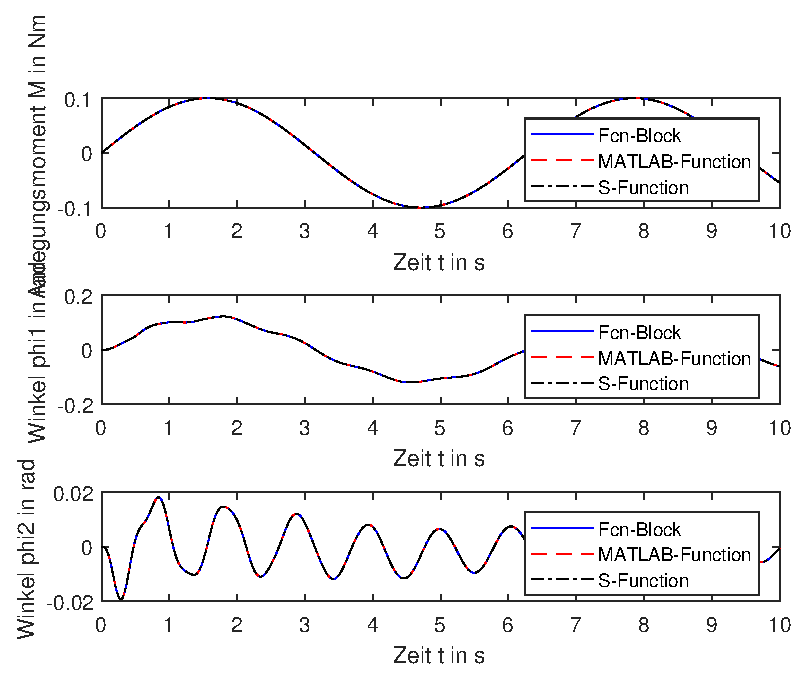
\includegraphics[width = \textwidth]{Bilder/V1_Modell_output_T10.eps}
	\caption{Vergleich der Modellierungsm�glichkeiten bei einer Simulationsdauer von 10s}
	\label{fig:Ergebnis_T10}
\end{figure}

\begin{figure}[!htb]
	\centering
	\includegraphics[width = \textwidth]{Bilder/V1_Modell_output_T2.eps}
	\caption{Vergleich der Modellierungsm�glichkeiten bei einer Simulationsdauer von 2s}
	\label{fig:Ergebnis_T2}
\end{figure}

Alle drei behandelten Modellierungsm�glichkeiten sind f�r die nichtlineare Modellierung geeignet. Bei gleicher Simulationseinstellung sind daher identische Ergebnisse zu erwarten. Wie die Abbildungen zeigen, erf�llen die Ergebnisse diese Erwartung.

Der Verlauf der Winkel in Abh�ngigkeit des Anregungssignals ist plausibel. F�r den Winkel $\varphi_1$ ist ein �hnlicher Verlauf wie das Anregungsmoment, nur mit einer kleiner Verz�gerung durch die Tr�gheitsmomente, zu erwarten, da das Anregungsmoment direkt auf die Drehachse in $\varphi_1$ wirkt und somit einen �hnlichen Verlauf erzwingt. Der Winkel $\varphi_2$ ist dagegen frei gelagert und ist nur durch ein Reibmoment begrenzt. Folglich ist anstatt eines zur Anregung synchronen Verlaufs ein frei schwingendes Verhalten zu erwarten. Das hei�t, dass der zweite Pendel auch in entgegengesetzter Richtung schwingen kann. Dies ist in der Darstellung der Ergebnisse f�r eine Simulationsdauer von 2s besonders am Anfang zu erkennen. Durch die Tr�gheit schwingt der zweite Pendel anf�nglich in die negative $\varphi_2$-Richtung. 

%Die D�mpfung, die durch die Reibmomente hervorgerufen wird, ist aus den Grafen nicht ersichtlich.


\end{document}
